\documentclass[t]{beamer}
\usetheme{Copenhagen}
\setbeamertemplate{headline}{} % remove toc from headers
\beamertemplatenavigationsymbolsempty

\usepackage{amsmath, tikz, bm, tkz-euclide,pgfplots}
\pgfplotsset{compat = 1.16}
\usetkzobj{all}
\everymath{\displaystyle}

\title{Rational Equations and Inequalities}
\author{}
\date{}

\AtBeginSection[]
{
  \begin{frame}
    \frametitle{Objectives}
    \tableofcontents[currentsection]
  \end{frame}
}

\begin{document}

\begin{frame} 
\maketitle
\end{frame}

\section{Solve rational equations}

\begin{frame}{Rational Equations}
In this section we will look at solving equations containing rational functions. \newline\\ \pause

Similar to the technique of simplifying complex fractions, we will eliminate our fractions by multiplying everything on both sides by the least common denominator.    \newline\\ \pause 

However, because our fractions contain variables in the denominator, we must remember that the denominator can never equal zero. \newline\\ \pause 

Thus, we must always check for extraneous solutions when solving rational equations and inequalities.  
\end{frame}

\begin{frame}{Example 1}
Solve each of the following. Remember to check for extraneous solutions.	\newline\\
(a)	\quad $\frac{1}{5x} = \frac{1}{5x^2} - \frac{x+5}{x^2}$
\onslide<2->{\qquad \alert{$x \neq 0$}} 
\onslide<3->{\qquad LCD is $5x^2$}
\begin{align*}
\onslide<4->{\left(5x^2\right)\left(\frac{1}{5x}\right) &= \left(\frac{1}{5x^2} - \frac{x+5}{x^2}\right)\left(5x^2\right)}	\\[10pt]
\onslide<5->{x &= 1-5(x+5)} \\[8pt]
\onslide<6->{x &= 1 - 5x - 25} \\[8pt]
\onslide<7->{6x &= -24} \\[8pt]
\onslide<8->{x &= -4}
\end{align*}
\end{frame}

\begin{frame}{Example 1}
(b)	\quad	$\frac{5}{3} - \frac{1}{x} = \frac{1}{3x}$
\onslide<2->{\qquad \alert{$x \neq 0$}} 
\onslide<3->{\qquad LCD is $3x$}
\begin{align*}
\onslide<4->{\left(3x\right)\left(\frac{5}{3} - \frac{1}{x}\right) &= \left(\frac{1}{3x}\right)\left(3x\right)}	\\[10pt]
\onslide<5->{5x-3 &= 1} \\[10pt]
\onslide<6->{x &= \frac{4}{5}}
\end{align*}
\end{frame}

\begin{frame}{Example 1}
(c)	\quad	$\frac{1}{x+4} = \frac{6x-42}{x^2+4x} + \frac{x-8}{x^2+4x}$
\onslide<2->{\[\frac{1}{x+4} = \frac{6(x-7)}{x(x+4)} + \frac{x-8}{x(x+4)}\]}	\\[4pt]
\onslide<3->{$x \neq 0, -4$}
\onslide<4->{\qquad LCD is $x(x+4)$}
\begin{align*}
\onslide<5->{\left(x(x+4)\right)\left(\frac{1}{x+4}\right) &= \left(\frac{6(x-7)}{x(x+4)} + \frac{x-8}{x(x+4)}\right)\left(x(x+4)\right)}	\\[10pt]
\onslide<6->{x &= 6(x-7)+x-8}	\\[8pt]
\onslide<7->{x &= 6x-42+x-8}
\end{align*}
\end{frame}

\begin{frame}{Example 1c	\quad $x \neq 0, -4$}
\begin{align*}
x &= 6x-42+x-8	\\[8pt]
\onslide<2->{x &= 7x-50} \\[8pt]
\onslide<3->{-6x &= -50} \\[10pt]
\onslide<4->{x &= \frac{25}{3}}
\end{align*}
\end{frame}

\begin{frame}{Example 1}
(d)	\quad	$\frac{1}{x^2-x} + \frac{1}{x} = \frac{5}{x^2-x}$
\onslide<2->{\[\frac{1}{x(x-1)} + \frac{1}{x} = \frac{5}{x(x-1)}\]}	\\[4pt]
\onslide<3->{$x \neq 0, -1$}
\onslide<4->{\qquad LCD is $x(x-1)$}
\begin{align*}
\onslide<5->{\left(x(x-1)\right)\left(\frac{1}{x(x-1)} + \frac{1}{x}\right) &= \left(\frac{5}{x(x-1)}\right)\left(x(x-1)\right)}	\\[10pt]
\onslide<6->{1 + x - 1 &= 5} \\[6pt]
\onslide<7->{x &= 5}
\end{align*}
\end{frame}

\begin{frame}{Example 1}
(e)	\quad	$1 = \frac{2}{x^2+x} + \frac{2}{x+1}$
\onslide<2->{\[1 = \frac{2}{x(x+1)} + \frac{2}{x+1}\]}	\\[4pt]
\onslide<3->{$x \neq 0, -1$} \onslide<4->{\qquad LCD is $x(x+1)$}
\begin{align*}
\onslide<5->{\left(x(x+1)\right)1 &= \left(\frac{2}{x(x+1)} + \frac{2}{x+1}\right)\left(x(x+1)\right)}		\\[10pt]
\onslide<6->{x^2+x &= 2 + 2x} \\[6pt]
\onslide<7->{x^2 - x - 2 &= 0} 
\end{align*}
\end{frame}

\begin{frame}{Example 1e \quad $x \neq 0, -1$}
\begin{align*}
x^2 - x - 2 &= 0		\\[8pt]
\onslide<2->{(x+1)(x-2) &= 0} \\[8pt]
\onslide<3->{x &= -1, \, 2} \\[8pt]
\end{align*}
Since $x \neq -1$ from the domain, our final answer is $x = 2$.
\end{frame}

\begin{frame}{Example 1}
(f)		\quad	$\frac{1}{3x-15} = \frac{1}{x^2-2x-15} + \frac{x^2}{3x^2-6x-45}$
\onslide<2->{\[\frac{1}{3(x-5)} = \frac{1}{(x-5)(x+3)} + \frac{x^2}{3(x-5)(x+3)}\]}		\\[4pt]
\onslide<3->{$x \neq 5, -3$} \onslide<4->{\qquad LCD is $3(x-5)(x+3)$}
\onslide<4->{\[\left(3(x-5)(x+3)\right)\left(\frac{1}{3(x-5)}\right) \onslide<5->{=x+3}\]}
\onslide<5->{\[\left(\frac{1}{(x-5)(x+3)} + \frac{x^2}{3(x-5)(x+3)}\right)\left(3(x-5)(x+3)\right)\]}
\onslide<6->{\[=3+x^2\]}
\end{frame}

\begin{frame}{Example 1f \quad $x \neq 5, -3$}
\begin{align*}
3+x^2 &= x + 3 \\[8pt]
\onslide<2->{x^2 - x &= 0} \\[8pt]
\onslide<3->{x(x-1) &= 0} \\[8pt]
\onslide<4->{x &= 0, \, 1}
\end{align*}
\end{frame}

\section{Solve rational inequalities}

\begin{frame}{Rational Inequalities}
We will continue the theme of solving inequalities like equations, setting up a number line, and using test values.    \newline\\

However, in addition to the answers we get from treating the inequality like an equation, we must also use the values outside the domain (i.e. where the denominator equals zero) on our number line.
\end{frame}

\begin{frame}{Example 2}
Solve each of the following and graph your solution on a number line.	\newline\\
(a)  \quad   $\frac{1}{5x} < \frac{1}{5x^2} - \frac{x+5}{x^2}$	\\[5pt]
\onslide<2->{\[\frac{1}{5x} = \frac{1}{5x^2} - \frac{x+5}{x^2}\]}	\\[5pt]
\onslide<3->{From Example 1a, we got $x=-4$ and $x \neq 0$}	\\[5pt]
\begin{center}
\onslide<4->{
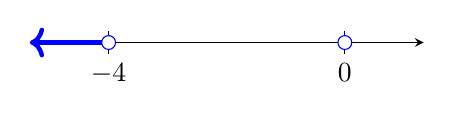
\begin{tikzpicture}
\draw [<->, >=stealth] (-2.5,0) -- (2.5,0);
\draw (-1.5,0.15) -- (-1.5,-0.15) node [below] {$-4$};
\draw (1.5,0.15) -- (1.5,-0.15) node [below] {$0$};
\onslide<5->{\draw[color=blue, fill=white] (-1.5,0) circle [radius=2.5pt];}
\onslide<6->{\draw[color=blue, fill=white] (1.5,0) circle [radius=2.5pt];}
\onslide<7->{\draw[color=blue, ultra thick, ->, shorten <=2.5pt] (-1.5,0) -- (-2.5,0);}
\end{tikzpicture}
}
\end{center}
\onslide<8->{\[x < - 4\]}
\end{frame}

\begin{frame}{Example 2}
(b)	\quad	$\frac{5}{3} - \frac{1}{x} \geq \frac{1}{3x}$
\onslide<2->{\[\frac{5}{3} - \frac{1}{x} = \frac{1}{3x}\]}	\\[5pt]
\onslide<3->{From Example 1b, we got $x=\frac{4}{5}$ and $x \neq 0$}	\\[5pt]
\begin{center}
\onslide<4->{
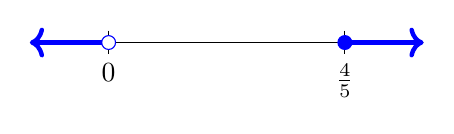
\begin{tikzpicture}
\draw [<->, >=stealth] (-2.5,0) -- (2.5,0);
\draw (-1.5,0.15) -- (-1.5,-0.15) node [below] {$0$};
\draw (1.5,0.15) -- (1.5,-0.15) node [below] {$\tfrac{4}{5}$};
\onslide<5->{\draw[color=blue, fill=white] (-1.5,0) circle [radius=2.5pt];}
\onslide<6->{\draw[color=blue, fill=blue] (1.5,0) circle [radius=2.5pt];}
\onslide<7->{\draw[color=blue, ultra thick, ->, shorten <=2.5pt] (-1.5,0) -- (-2.5,0);
\draw[color=blue, ultra thick, ->, shorten <=2.5pt] (1.5,0) -- (2.5,0);}
\end{tikzpicture}
}
\end{center}
\onslide<8->{\[x < 0 \text{\quad or \quad} x \geq \frac{4}{5}\]}
\end{frame}

\begin{frame}{Example 2}
(c)	\quad	$\frac{1}{x+4} \leq \frac{6x-42}{x^2+4x} + \frac{x-8}{x^2+4x}$
\onslide<2->{\[\frac{1}{x+4} = \frac{6x-42}{x^2+4x} + \frac{x-8}{x^2+4x}\]}	\\[5pt]
\onslide<3->{From Example 1c, we got $x=\frac{25}{3}$ and $x \neq 0, \, -4$}	\\[5pt]
\begin{center}
\onslide<4->{
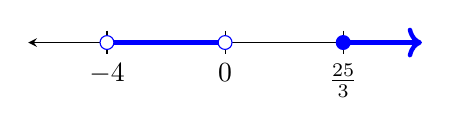
\begin{tikzpicture}
\draw [<->, >=stealth] (-2.5,0) -- (2.5,0);
\draw (-1.5,0.15) -- (-1.5,-0.15) node [below] {$-4$};
\draw (0,0.15) -- (0,-0.15) node [below] {$0$};
\draw (1.5,0.15) -- (1.5,-0.15) node [below] {$\tfrac{25}{3}$};
\onslide<5->{\draw[color=blue, fill=white] (-1.5,0) circle [radius=2.5pt];}
\onslide<6->{\draw[color=blue, fill=blue] (1.5,0) circle [radius=2.5pt];}
\onslide<5->{\draw[color=blue, fill=white] (0,0) circle [radius=2.5pt];}
\onslide<7->{\draw[color=blue, ultra thick, shorten <=2.5pt, shorten >=2.5pt] (-1.5,0) -- (0,0);
\draw[color=blue, ultra thick, ->, shorten <=2.5pt] (1.5,0) -- (2.5,0);}
\end{tikzpicture}
}
\end{center}
\onslide<8->{\[-4 < x < 0 \text{\quad or \quad} x \geq \frac{25}{3}\]}
\end{frame}

\begin{frame}{Example 2}
(d)	\quad	$\frac{1}{x^2-x} + \frac{1}{x} > \frac{5}{x^2-x}$
\onslide<2->{\[\frac{1}{x^2-x} + \frac{1}{x} = \frac{5}{x^2-x}\]}	\\[5pt]
\onslide<3->{From Example 1d, we got $x=5$ and $x \neq 0, \, 1$}	\\[5pt]
\begin{center}
\onslide<4->{
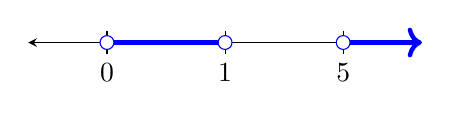
\begin{tikzpicture}
\draw [<->, >=stealth] (-2.5,0) -- (2.5,0);
\draw (-1.5,0.15) -- (-1.5,-0.15) node [below] {$0$};
\draw (0,0.15) -- (0,-0.15) node [below] {$1$};
\draw (1.5,0.15) -- (1.5,-0.15) node [below] {$5$};
\onslide<5->{\draw[color=blue, fill=white] (-1.5,0) circle [radius=2.5pt];}
\onslide<5->{\draw[color=blue, fill=white] (1.5,0) circle [radius=2.5pt];}
\onslide<5->{\draw[color=blue, fill=white] (0,0) circle [radius=2.5pt];}
\onslide<7->{\draw[color=blue, ultra thick, shorten <=2.5pt, shorten >=2.5pt] (-1.5,0) -- (0,0);
\draw[color=blue, ultra thick, ->, shorten <=2.5pt] (1.5,0) -- (2.5,0);}
\end{tikzpicture}
}
\end{center}
\onslide<8->{\[0 < x < 1 \text{\quad or \quad} x > 5\]}
\end{frame}

\begin{frame}{Example 2}
(e)	\quad	$1 \leq \frac{2}{x^2+x} + \frac{2}{x+1}$
\onslide<2->{\[1 = \frac{2}{x^2+x} + \frac{2}{x+1}\]}	\\[5pt]
\onslide<3->{From Example 1e, we got $x=2$ and $x \neq 0, \, -1$}	\\[5pt]
\begin{center}
\onslide<4->{
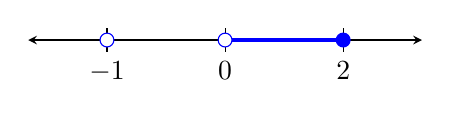
\begin{tikzpicture}
\draw [<->, >=stealth] (-2.5,0) -- (2.5,0);
\draw (-1.5,0.15) -- (-1.5,-0.15) node [below] {$-1$};
\draw (0,0.15) -- (0,-0.15) node [below] {$0$};
\draw (1.5,0.15) -- (1.5,-0.15) node [below] {$2$};
\onslide<5->{\draw[color=blue, fill=white] (-1.5,0) circle [radius=2.5pt];}
\onslide<6->{\draw[color=blue, fill=blue] (1.5,0) circle [radius=2.5pt];}
\onslide<5->{\draw[color=blue, fill=white] (0,0) circle [radius=2.5pt];}
\onslide<7->{\draw[color=blue, ultra thick, shorten <=2.5pt, shorten >=2.5pt] (0,0) -- (1.5,0);}
\end{tikzpicture}
}
\end{center}
\onslide<8->{\[0 < x \leq 2\]}
\end{frame}

\begin{frame}{Example 2}
(f)		\quad	$\frac{1}{3x-15} \geq \frac{1}{x^2-2x-15} + \frac{x^2}{3x^2-6x-45}$
\onslide<2->{\[\frac{1}{3x-15} = \frac{1}{x^2-2x-15} + \frac{x^2}{3x^2-6x-45}\]}	\\[5pt]
\onslide<3->{From Example 1f, we got $x=0, \, 1$ and $x \neq 5, \, -3$}	\\[5pt]
\begin{center}
\onslide<4->{
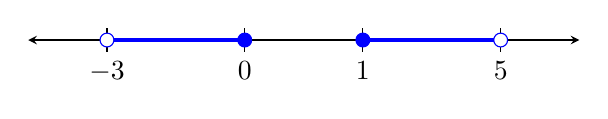
\begin{tikzpicture}
\draw [<->, >=stealth] (-3.5,0) -- (3.5,0);
\draw (-2.5,0.15) -- (-2.5,-0.15) node [below] {$-3$};
\draw (-0.75,0.15) -- (-0.75,-0.15) node [below] {$0$};
\draw (0.75,0.15) -- (0.75,-0.15) node [below] {$1$};
\draw (2.5,0.15) -- (2.5,-0.15) node [below] {$5$};
\onslide<5->{\draw[color=blue, fill=white] (-2.5,0) circle [radius=2.5pt];}
\onslide<6->{\draw[color=blue, fill=blue] (0.75,0) circle [radius=2.5pt];}
\onslide<6->{\draw[color=blue, fill=blue] (-0.75,0) circle [radius=2.5pt];}
\onslide<5->{\draw[color=blue, fill=white] (2.5,0) circle [radius=2.5pt];}
\onslide<7->{\draw[color=blue, ultra thick, shorten <=2.5pt, shorten >=2.5pt] (-2.5,0) -- (-0.75,0);
\draw[color=blue, ultra thick, shorten <=2.5pt, shorten >=2.5pt] (0.75,0) -- (2.5,0);}
\end{tikzpicture}
}
\end{center}
\onslide<8->{\[-3 < x \leq 0 \text{\quad or \quad} 1 \leq x < 5\]}
\end{frame}

\end{document}